\section{Redondances dans les règles}\label{sec:regles}

\begin{definition}[frontière]
La frontière d'une règle est l'ensemble des variables appartenant à la fois au corps et à la tête de la règle. On le note $fr(R)$.
\end{definition}\label{def:frontier}

\begin{definition}[Pièce dans une règle]
    On appelle pièce d’une règle une pièce de la tête de la règle (la tête étant un ensemble d'atomes).
\end{definition}

\begin{example}
   Soit la regle $R= p(x, y),p(y, t) \rightarrow r(x,z),r(z,u),q(u),s(x, y, v), q(y)$\\
    On peut décomposer chaque règle $R$ en un ensemble de règles dont la tête n’a qu’une seule pièce, chacune ayant le même corps que $R$. \\On aura,
    \begin{itemize}
        \item[*]$R_1= p(x, y),p(y, t) \rightarrow r(x,z),r(z,u),q(u)$
      \item[*]$R_2= p(x, y),p(y, t) \rightarrow s(x, y, v), q(y)$
    \end{itemize}
    Une règle  dont la tête n’a qu’une seule pièce est dit règle monopièce.
\end{example}

\begin{definition}[Redondance dans le corps de la règle]\label{def:body_redundancy}
    Soit $R = B \rightarrow H$ une règle, $R' = frontierFreeze(R) = (B' \rightarrow H')$ et $\alpha \in B'$. On dit qu'il existe une redondance dans $B$ si et seulement si, il existe un homomorphisme : $h : \alpha \mapsto B'\setminus\{\alpha\}$. 
    Il y a absence de redondances dans le corps si il n'existe pas de tel $\alpha$.
\end{definition}

\begin{example}
    Soit une règle $r = p(X,Y) \land p(X,b) \rightarrow p(Z,X)$. L'atome $p(X,Y)$ est redondant car il existe un homomorphisme $h = \{(X \mapsto X), (Y \mapsto b)\}$ tel que $h(p(X,Y)) = p(X,b)$.
\end{example}

\begin{definition}[Redondance dans la tête de la règle] \label{def:head_redundancy}
Soit $R = B \rightarrow H$ une règle, $R' = frontierFreeze(R) = (B' \rightarrow H')$ et $\alpha \in H'$. On dit qu'il existe une redondance dans $H$ si et seulement si, il existe un homomorphisme : $h : \alpha \mapsto H'\setminus\{\alpha\}$.  
Il y a absence de redondances dans la tête si il n'existe pas de tel $\alpha$.
\end{definition}

\begin{example}
    Soit une règle $r = p(X,Y) \rightarrow p(Z,X)\land p(W,X) $. L'atome $p(W,X)$ est redondant car il existe un homomorphisme $h = \{(X \mapsto X), (W \mapsto Z)\}$ tel que $h(p(W,X)) = p(Z,X)$.
\end{example}

\begin{definition}[Redondance de la tête dans le corps de la règle]\label{def:headToBody_redundancy}
 Soit $R = B \rightarrow H$ une règle, $R' = frontierFreeze(R) = (B' \rightarrow H')$ et $\alpha \in H'$. On dit qu'il existe une redondance de la tête $H$ sur le corps $B$, si et seuleuement si il existe un homomorphisme : $h : \alpha \mapsto B'$.
 Il y a absence de redondances dans de la tête sur le corps d'une règle quand il n'existe pas un tel $\alpha$.
\end{definition}

\begin{definition}[Redondance de la tête dans le corps et la tête de la règle]\label{def:headToBodyAndHead_redundancy}
 Soit $R = B \rightarrow H$ une règle, $R' = frontierFreeze(R) = (B' \rightarrow H')$ et $\alpha \in H'$. On dit qu'il existe une redondance de la tête $H$ sur le corps $B$ et la tête $H$, si et seuleuement si il existe un homomorphisme : $h : \alpha \mapsto B' \cup H'$.
 Il y a absence de redondances dans de la tête sur le corps d'une règle quand il n'existe pas un tel $\alpha$.
\end{definition}

\begin{example}
Soit la règle $r = p(X, Y) \rightarrow \exists Z, p(X, Z)$.
\par $p(X,Z)$ est redondant par rapport à $p(X,Y)$ : on sait qu'il existe un tel $Z$, il s'agit de $Y$. Il existe donc un homomorphisme $h = \{(X\mapsto X), (Z \mapsto Y)\}$ tel que $h(p(X,Z)) = p(X,Y)$.

\end{example}

\par À partir d'un ensemble d'atomes on peut supprimer les atomes redondants de cet ensemble à l'aide du calcul du \textit{Core} (def. \ref{def:Core}).
Si on a une règle $(B \rightarrow H)$ dont on a gelé la frontière. En utilisant le corps de la règle comme ensemble d'atomes on va pouvoir supprimer ce qui est redondant. De même pour la tête.
\par On peut donc aussi considérer l'ensemble $freeze(B, H)$ (def. \ref{def:freeze()}). Comme les atomes du corps $B$ sont gelés et la frontière de la règle aussi le \textit{Core} essaiera de replier les atomes de la tête sur les atomes de la tête et du corps. Ce calcul inclus donc la suppression de redondance de la tête dans la tête (def. \ref{def:head_redundancy}).

%\begin{proposition}
    
%Soit une règle $R$. Alors si on gèle le corps de la règle, on peut appliquer l'algorithme du calcul du $Core$ sur $R$ pour supprimer les redondances. 
%\end{proposition}



\begin{proposition}
Le calcul du $Core$ de $G$ associé à la règle $R$ ne supprime que des redondances.
\end{proposition}

%\begin{proof}
%D'après la définition du $Core$ (def. \ref{def:Core}).
%\end{proof}


\begin{itemize}
    \item Tout d'abord, on va appliquer une transformation des règles $R \in \mathcal{R}$ qui va supprimer les redondances dans son \textit{corps} et dans sa \textit{tête} ;
    \item Ensuite, on appelle la procédure \textit{RuleCore} à $R'$ (algorithme \ref{algo:ruleCore}) ;  
    \item Enfin, on ajoute $R'$ dans la nouvelle base de règle $\mathcal{R'}$.
\end{itemize}


\setstretch{1}
\begin{algorithm}[H]\label{algo:redondances}
\caption{Suppression de redondances}
\SetAlgoLined
\DontPrintSemicolon
\SetAlgoLined
\DontPrintSemicolon
\SetKwInOut{Input}{entrées}
\SetKwInOut{Output}{sortie}
\Input{une base de règles $\mathcal{R}$}
\Output{la base de règles $\mathcal{R'}$}
% suppression dans le coprs -> freeze du corps -> Core -> defreeze
    $\mathcal{R}' \gets \{\}$\; 
    \ForEach{$ R = B \rightarrow  H \in \mathcal{R}$} 
    {
        $R' \gets $ \textit{créerRègle(Core(frontierFreeze(B)) , H)} \;
        $R' \gets RuleCore(R')$\;
        $\mathcal{R'} \gets \mathcal{R'} \cup \{R'\}$\;
    }
    \Return $\mathcal{R}'$
\end{algorithm}
%
%\paragraph{Le \textit{BodyChecker}}
%Le \textit{BodyChecker} supprime ce qui est redondant dans le \textit{corps} d'une règle $R$. Il va d'abord geler la frontière sur $R$. Ensuite on calcule le $Core$ du \textit{corps} de $R$. Enfin on dégèle $R$. 
%\newline

%\setstretch{1}
%\begin{algorithm}[H]\label{algo:bodyChecker}
%%\caption{Body Checker} 
%\SetAlgoLined
%\DontPrintSemicolon
%%\SetAlgoLined
%\DontPrintSemicolon
%\SetKwInOut{Input}{entrées}
%\SetKwInOut{Output}{sortie}
%\SetKwInOut{Variables}{Variables}
%\Input{une règle $R = B \rightarrow  H$}
%\Output{la règle $R$ sans redondance dans $B$}
% frontierfreeze  -> Core sur le body 
 %   $frontierFreeze(R)$\;  
 %   $B' \gets Core(B)$\;
 %   $R' \gets (B' \rightarrow H)$\;
 %   $unfreeze(R')$\;
 %   \Return $R'$
%\end{algorithm}

\paragraph{Le \textit{RuleCore}}
Le \textit{RuleCore} va supprimer ce qui est redondant dans la \textit{tête} et de la \textit{tête} sur le \textit{corps} d'une règle. On va geler (\ref{def:freeze()}) les variables dans $B$ qui sont dans $R$, on obtient $F$ qui est un ensemble d'atomes. Enfin on applique le calcul du $Core$ à $F$ pour obtenir $F'$ sans atomes redondant. Pour finir on construit $R'$ à partir de $F'$ et on retourne $R'$.
\newline


\setstretch{1}
\begin{algorithm}[H]\label{algo:ruleCore}
\caption{Rule Core} %revoir le nom
\SetAlgoLined
\DontPrintSemicolon
\SetAlgoLined
\DontPrintSemicolon
\SetKwInOut{Input}{entrées}
\SetKwInOut{Output}{sortie}
\SetKwInOut{Variables}{Variables}
\Input{une règle $R = B \rightarrow  H$}
\Output{la règle $R'$}
% suppression dans le coprs -> freeze du corps -> Core -> defreeze
    $H', F, F'\gets \{\} $ // ensemble d'atomes\;
    $F \gets freeze(B, H)$\;
   
    $F' = Core(F)$\;
    \ForEach{$\alpha \in F'$} 
    {
        \uIf{$\alpha \notin B$}
        {
            $H' \gets defreeze(\{\alpha\})$\;
        }
    }
    $R' \gets (B \rightarrow H')$\;

    \Return $R'$
\end{algorithm}

\begin{definition}
    Soit $\mathcal{R}$ une base de règle et $R \in \mathcal{R}$ une règle. On dit que $R$ est redondante dans $\mathcal{R}$ si et seulement si $\mathcal{R} \backslash\{R\} \vDash R$.
\end{definition}

\paragraph{Le \textit{SimpleRules}}
Le \textit{SimpleRules} va supprimer toutes les règles $R$ redondantes par rapport à une base de règle $\mathcal{R}$. Pour chaque règle $R$ on va utiliser un algorithme de chaînage avant appliqué sur une base de connaissance qui a pour base de fait le corps de la règle $R$ à tester et pour base de règle : $\mathcal{R} \backslash \{R\}$. Si la tête de la règle $H$ est présente dans la base de faits saturées alors on a $\mathcal{R} \backslash \{R\} \models R$. Donc $R$ est redondante par rapport à $\mathcal{R}$. Sinon on maintient $R$ dans $\mathcal{R}$. 
\newline



\setstretch{1}
\begin{algorithm}[H]\label{algo:rule}
\caption{SimpleRules} %revoir le nom
\SetAlgoLined
\DontPrintSemicolon
\SetAlgoLined
\DontPrintSemicolon
\SetKwInOut{Input}{entrées}
\SetKwInOut{Output}{sortie}
\SetKwInOut{Variables}{Variables}
\Input{une base de règles $\mathcal{R}$}
%\Output{la règle $R'$}
\Output{La base de règles $\mathcal{R}'$ non redondante}
% pour chaque regle on verifie si R \ r |= r
% freeze des base regle \ r et chercher un homomorphisme de r dans base regle     
    \ForEach{$r = B \rightarrow H \in \mathcal{R}$} 
    {
         $\mathcal{F} \gets$ créerFactBase($freeze$($B$))\;
         $\mathcal{F}^* \gets$ Chase($\mathcal{F}$, $\mathcal{R} \backslash \{r\}$)\;
         \uIf{\textit{il existe un homomorphisme }$ h : B \rightarrow \mathcal{F}^*$ et qu'il existe une extension $h_s : H \rightarrow \mathcal{F}^*$ de $h$}
        {
            $\mathcal{R} \gets \mathcal{R} \backslash \{r\}$\;
        }
    }
    \Return $\mathcal{R}$
\end{algorithm}

    \subsection{Analyse du nouveau travail dans Graal}
        \begin{figure}[H]
        \centering
        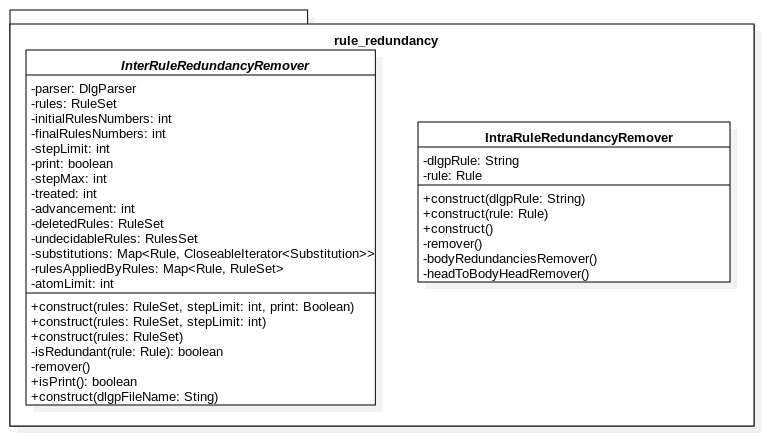
\includegraphics[width=\textwidth]{pictures/RedondanceDiagrammeClasse.png}
        \caption{Diagramme de classes pour les redondances des règles}
        \label{fig:dclasse}
        \end{figure}
        
    \paragraph{Package Rule Redundancy}
         \begin{itemize}
            \item Redundancy : Interface à implémenter pour toutes les classes de redondance sur les règles. 
            \item HeadToBodyRedundancyRemover : Classe qui élimine la redondance dans une règle.
            \item RuleSetRedundancy : Classe qui élimine les règles redondantes dans un ensemble de règles.
            \item RuleApplierForRuleRedundancy : Classe qui permet de savoir tous les homomorphismes et les règles appliquées.
        \end{itemize}
        
    \paragraph{Classe HeadToBodyRedundancyRemover}\ \\
         On applique dans cette classe l'algorithme \ref{algo:redondances} pour la suppression de redondances dans les règles. Cet algorithme va prendre chaque règle du $\mathcal{BR}$ et va supprimer les redondances dans son \textit{corps} et puis dans sa \textit{tête} et de la \textit{tête} sur son \textit{corps}.
         
    \paragraph{Classe RuleSetRedundancy}\ \\
         On applique dans cette classe l'algorithme \ref{algo:rule} pour la suppression des règles redondantes dans une base de règles donnée. Cet algorithme va tester chaque règle de la base de règles $\mathcal{BR}$ pour vérifier si elle est redondante par rapport à $\mathcal{BR}$, si c'était le cas on la retire de $\mathcal{BR}$ et sinon il faut la laisser.
         
    \paragraph{Classe MainRedundancy}\ \\
         Pour l'application des algorithmes d'élimination de redondances des règles on a créer la classe \textit{MainRedundancy} qui prend une ontologie en format \textit{.dlp} et selon les paramètres données on applique l'élimination de redondance dans chacune des règles (phase 1), pour chaque règle par rapport à tous les règles (phase 2) ou les deux (phase 1 et 2). Une nouvelle bases de règles va être créer, à la fin de l'exécution, dans un fichier \textit{.dlp}. Pour avoir les détails de chaque exécution, un fichier \textit{.txt} sera créer. Ce fichier va contenir les informations nécessaires pour la simplification de chaque règle dans la phase 1, de plus les homomorphismes et les règles utilisés pour justifier la redondance de la règle à éliminer.